\documentclass{zbc-report}

\usetikzlibrary{shapes.geometric}  % Including shapes.geometric for TikZ
\usepackage[normalem]{ulem}
\useunder{\uline}{\ul}{}

%% Set up the bibliography
\usepackage{biblatex}
\addbibresource{report.bib}

%% Additional packages and commands
\usepackage{parskip}
\setlist{itemsep=-2pt} % Reducing white space in lists slightly
\renewcommand{\deg}{\si{\degree}\xspace} % Use \deg easily, everywhere

%% Set up the minted package
\usepackage[cachedir=_minted-report]{minted}
\setminted{
    linenos=true,
    breaklines=true,
    fontsize=\footnotesize,
    frame=lines,
    framesep=2mm,
    baselinestretch=1.2,
    bgcolor=gray!10,
    style=vs,
    mathescape=true,
}

%% ----------------------------------------------------------------------
%%    Begin of document + Frontmatter (Roman page numbering)
%% ----------------------------------------------------------------------

\begin{document}

\frontmatter

%% Define the main parameters
\title{Semesterproject Webshop}
\subtitle{Computer Science\\ 2nd Semester}
\author{Carsten Lydeking}

\subject{Software Design and Construction} % Cover only
\large\affiliation{Zealand Business College} % Cover only
\coverimage{figures/template-figures/binary.jpg} % Aspect ratio of 2:3 (portrait) recommended
\definecolor{title}{HTML}{4884d6} % Color for cover title

\makecover

\begin{titlepage}

\begin{center}

%% Print the title
{\makeatletter
\largetitlestyle\fontsize{45}{45}\selectfont\@title
\makeatother}

%% Print the subtitle
{\makeatletter
\ifdefvoid{\@subtitle}{}{\bigskip\titlestyle\fontsize{20}{20}\selectfont\@subtitle}
\makeatother}

\bigskip
\bigskip

%% Print the name of the author
{\makeatletter
\largetitlestyle\fontsize{25}{25}\selectfont\@author
\makeatother}

\bigskip
\bigskip

%% Print table with names and student numbers
\setlength\extrarowheight{2pt}
\begin{tabular}{c}
    cal002@edu.zealand.dk \\
\end{tabular}

\vfill

%% Print some more information at the bottom
\begin{tabular}{l r}
    Lecturer, SWC:    & Henrik Kryger Høltzer\\
    Lecturer, SWD:    & Mikkel Lynggaard Krarup\\
    Project Deadline: & \ddmmyydate{30/05/24} \\
    Handed-in:       & \ddmmyydate{\today} \\
    Faculty:         & Computer Science \\
    Semester:        & 2nd Semester \\
    Word Count:      & 48180 Characters (including spaces) \\
\end{tabular}

\bigskip
%% Add a source and description for the cover and optional attribution for the template
\begin{tabular}{l r}
    Cover: & Generated image of binary using DALL-E \\
    Style: & ZBC template -- created by Carsten Lydeking \\
\end{tabular}


%% Insert the Zealand logo at the bottom of the page
\begin{tikzpicture}[remember picture]
    \node[above=10mm] at (current page.south) {%
        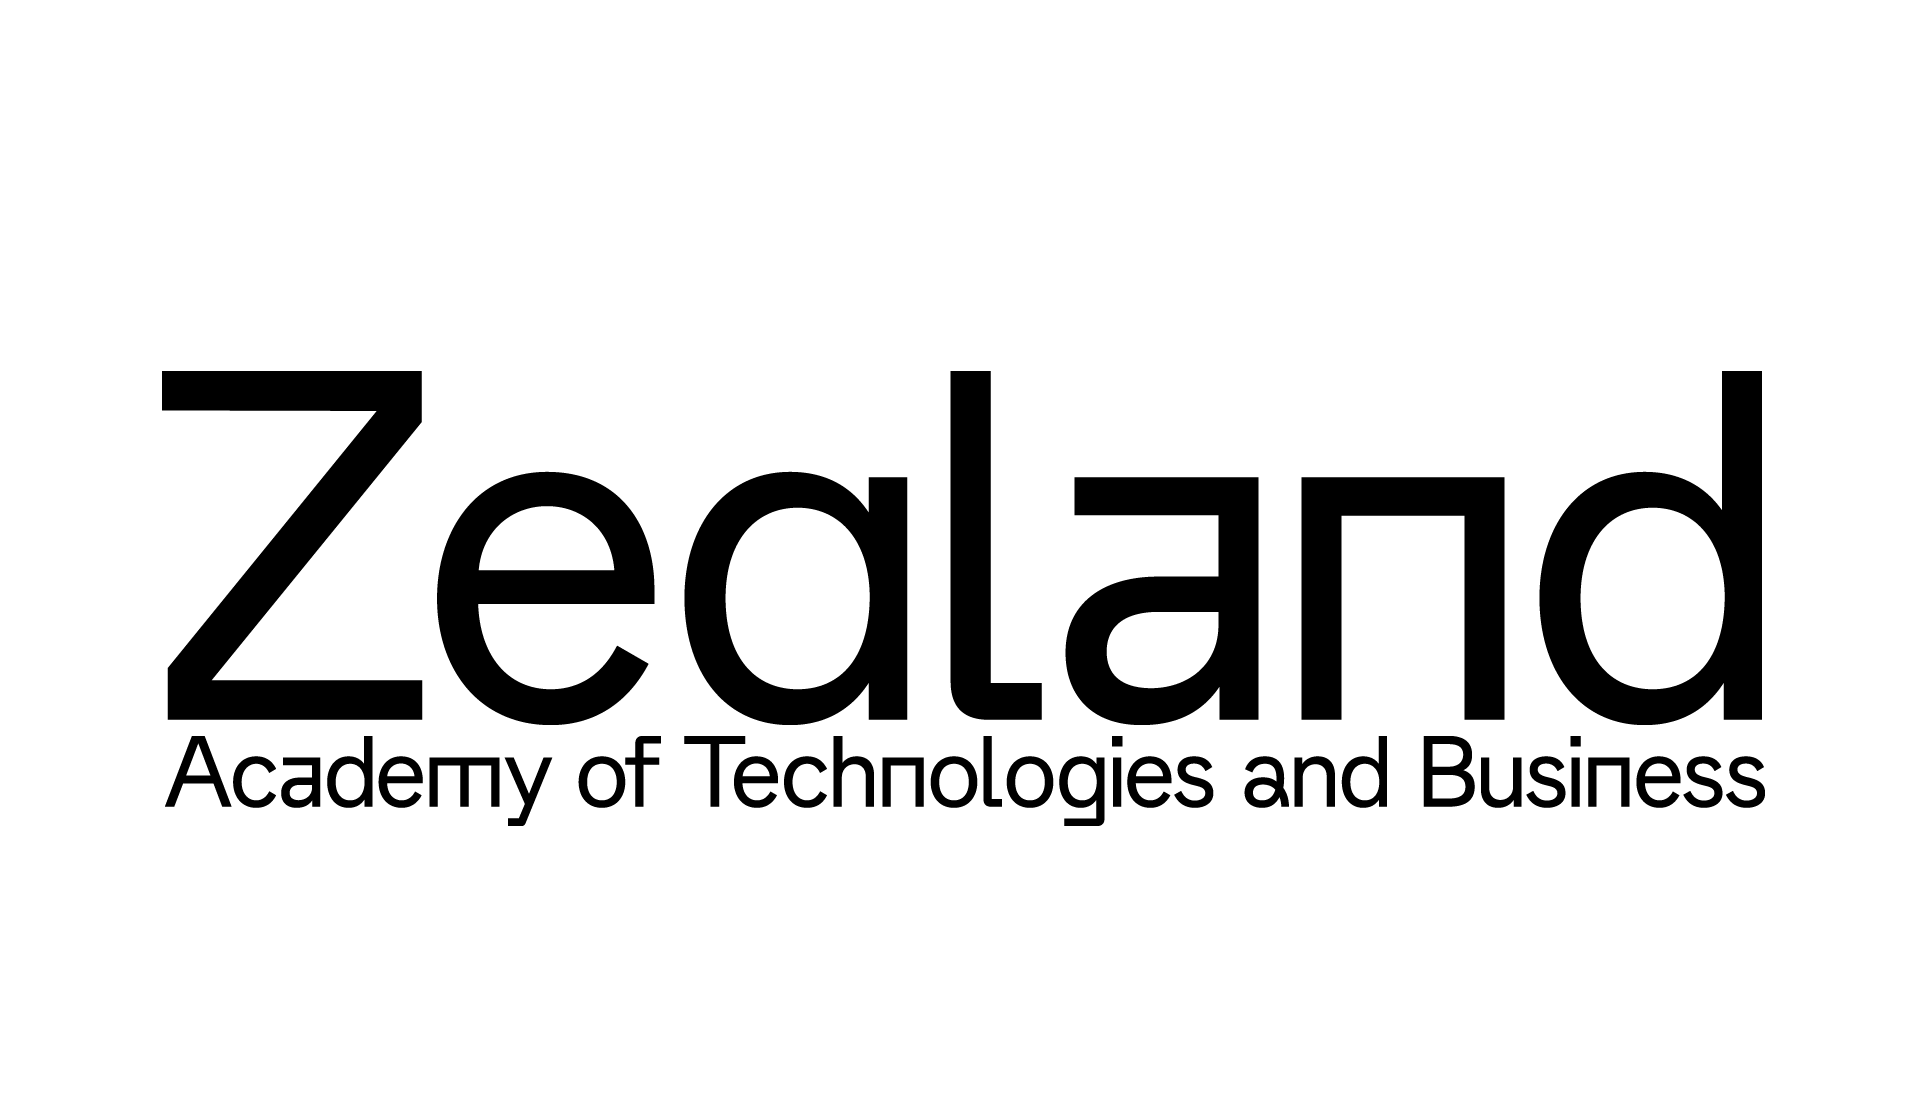
\includegraphics[width=0.35\textwidth]{figures/template-figures/zealandcombinedlogo}
    };
\end{tikzpicture}

\end{center}

\end{titlepage}

\tableofcontents
\listoffigures
\listoftables

%\chapter*{Nomenclature}
\addcontentsline{toc}{chapter}{Nomenclature}

\section{Abbreviations and definitions}
\label{sec:abbreviations}
The following abbreviations and definitions are used throughout the report:

\renewcommand{\arraystretch}{2}
\begin{longtable}{l p{13.5cm}}
    \textbf{Abb.}  & \textbf{Definition}  \\ \hline
        DB           & Database: A structured collection of data stored electronically. \\ \hline
        RDB          & Relational Database: A type of DB that stores and provides access to data points that are related to one another. \\ \hline
        DBMS         & Database Management System: Software that handles the storage, retrieval, and updating of data in a database. \\ \hline
        RDBMS        & Relational DBMS: A database management system based on the relational model introduced by E.F. Codd. \\ \hline
        SQL          & Structured Query Language: A programming language used to manage and manipulate relational databases. \\ \hline
        CRUD         & Create, Read, Update, Delete The four basic operations of persistent storage: adding, retrieving, modifying, and removing data. \\ \hline
        GUI          & Graphical User Interface  A user interface that allows users to interact with electronic devices using graphical icons and visual indicators. \\ \hline
        PK           & Primary Key:A unique identifier for each record in a database table. \\ \hline
        FK           & Foreign Key: A field in a database table that links to the primary key of another table. \\ \hline
        NML          & Normalization: In relation to RDB design, the process of organizing the columns (attributes) and tables (relations) to minimize data redundancy. \\ \hline
        1NF          & First Normal Form: A stage of NML where each table has atomic (i.e. indivisible) values and each record needs to be unique. \\ \hline
        2NF          & Second Normal Form: A stage of NML where it meets all the requirements of the 1NF and does not have partial dependency. \\ \hline
        3NF          & Third Normal Form: A stage of NML where it meets all the requirements of the 2NF and has no transitive functional dependencies. \\ \hline
        ERD          & Entity Relationship Diagram: A graphical representation of entities and their relationships to each other, typically used in database design. \\ \hline
        UML          & Unified Modeling Language: A standardized modeling language used to specify, visualize, construct, and document the artifacts of software systems. \\ \hline
        DDL          & Data Definition Language: A subset of SQL used to define database structures, such as tables, schemas, and databases. \\ \hline
        DML          & Data Manipulation Language: A subset of SQL used for adding (inserting), deleting, and modifying (updating) data in a database. \\ \hline
        DCL          & Data Control Language: A subset of SQL used to control access to data in a database. \\ \hline
        TCL          & Transaction Control Language: A subset of SQL used to manage the changes made by DML statements. \\ \hline
        XML          & Extensible Markup Language: A markup language that defines a set of rules for encoding documents in a format that is both human-readable and machine-readable. \\ \hline
        JSON         & JavaScript Object Notation: A lightweight data-interchange format that is easy for humans to read and write, and for machines to parse and generate. \\ \hline
    \renewcommand{\arraystretch}{1}
\end{longtable}

%% ----------------------------------------------------------------------
%%    Mainmatter (Arabic page numbering)
%% ----------------------------------------------------------------------

\mainmatter

\chapter{Introduction}
\label{chapter:introduction}

\section{Case}
\label{sec:case}
So what is the case?

\begin{itemize}
	\item an item
	\item another item
	\item yet another item
\end{itemize}

\section{Project description}
\label{sec:project_description}

\subsection{Problem statement}
\label{sec:problem_statement}
What is the problem?

\subsection{Problem analysis}
\label{sec:problem_analysis}

\subsection{Purpose}
\label{sec:purpose}

\subsection{Goal}
\label{sec:goal}

\subsection{Scope}
\label{sec:scope}

\section{Method}
\label{sec:method}

\chapter{2nd Chapter}
\label{chapter:2ndchapter}

This is the second chapter.

\section{SCRUM}
I think that \emph{SCRUM} is .. this is a reference \cref{fig:appendix-domain-model-diagram}.

\subsubsection{This is a subsubsection}
This is a subsubsection text, this is a cite \cite{connolly2023database}.
\input{mainmatter/chapter-3}
\input{mainmatter/chapter-4}
\input{mainmatter/chapter-5}
\input{mainmatter/chapter-6}
\input{mainmatter/chapter-7}

\chapter{Konklusion}
\label{chapter:conclusion}

\section{Opsummering}
\label{sec:conclusion_summary}

\subsection{Forretningsanalyse}
Gennem diverse modeller og analyser blev der grundlagt en solid forståelse af stakeholders' egne ønsker samt, hvad projektet yderligere kunne bidrage af værdi. 
Ud fra dette skulle der udformes \emph{User Stories}, som kunne bidrage til, at projektet holdt kursen mod et godt produkt. 
Ydermere var der overvejelser om, hvilke dele og funktionaliteter der først skulle flyttes \emph{out-of-scope}, hvis der opstod modstand i løbet af processen.
Det blev vurderet, at projektet var \emph{viable} ud fra de stillede parametre og foranstaltninger. 

\subsection{SCRUM}
\emph{SCRUM}-processen blev brugt til at strukturere projektet og sikre, at der blev leveret funktionalitet til tiden.
\emph{Trello} blev anvendt til at holde styr på processen og dokumentere arbejdet.
Der blev brugt \emph{Workflows}, der gav input til \emph{User Stories} og \emph{Mapping}. Hver \emph{User Story} fik \emph{Tasks}, \emph{Acceptance Criteria} og et \emph{Story Point} estimat.
Herfra blev der lavet en prioriteret \emph{Product Backlog}, der blev brugt til at planlægge \emph{Sprints}, som blev yderligere raffineret.
Gennem iterationer af \emph{Daily Standups}, \emph{Sprint Reviews} og \emph{Retrospectives} - som var modificeret til omstændighederne - blev processen udviklet og optimeret.

\subsection{Software Design}
Der blev udarbejdet en række modeller, der beskrev systemets struktur og funktionalitet. Kernemodellerne har understøttet udviklingen af systemet og har været retningsgivende for implementeringen.
De har dog alle undergået en række ændringer i løbet af projektet for at tilpasse sig systemets udvikling og de krav, der opstod undervejs.
Der blev lagt vægt på at designe et system, der var fleksibelt og kunne udvides med nye funktionaliteter. Bl.a. at en \emph{Employee} har en \emph{Salary}, der senere kan bruges i et lønsstyringsmodul.
Samtidig var brugervenlighed og det intuitive design indtænkt, så brugerne kunne finde rundt og bruge systemet uden problemer.
Hertil kom også overvejelser omkring sikkerhed og performance, der blev indtænkt i designet. \emph{Unit tests} blev anvendt i mindre omfang.
Den dokumentation, der blev udarbejdet, har været lavet med den hensigt, at en læser kan forstå kernedele af systemet og dets funktionalitet uden at have været med i udviklingsprocessen.
Der er dog ikke fuld dokumentation eller test, der beskriver alle aspekter af systemet, da det ville være for omfattende og ikke nødvendigt for projektet.
Prioriteringen er med henblik på at have en enkelt udvikler, der har siddet med alle dele af projektet.
Der har dog været eksperimenteret med bl.a. \emph{Doxygen} for at kunne generere dokumentation.

\subsection{SCRUM Dokumentation}
Der blev anvendt en tilpasset version af \emph{SCRUM}, der passede til projektets størrelse og sammensætning. Mange af elementerne har været modificeret, da \emph{SCRUM} ikke måtte blive en hindring for projektet.
Forventningerne forud for projektet var, at der ville være store overlap mellem \emph{Sprints}, at der ville være \emph{User Stories}, der ikke blev færdiggjort, at der ville være en del \emph{User Stories}, der blev fejlestimeret, og at \emph{Burndown Chartet} ville ligne Teslas aktiekurs.
Det har ikke været oplevelsen, hvilket kan tilskrives forskellige faktorer. Bl.a. var projektet relativt kortvarigt og relativt overskueligt. 
Kombineret med at estimeringsintervallet kun bestod af fem værdier med et begrænset numerisk interval, så var det svært at lave voldsomme fejlestimeringer. 
Det bør også faktoreres ind, at der kun var en enkelt udvikler, som havde en rimelig forståelse af egne kompetencer, samt at der ikke var indblandet en \emph{Product Owner}, der kunne have skabt større udfordringer.
Med rette kan det derfor diskuteres, om estimeringerne var brugbare, om overskueligheden kom fra et ensidigt synspunkt med kun en udvikler, og om det i det hele taget var nødvendigt at have en så omfattende proces.
Samtidig kan det overvejes, om der kunne være nået mere på selve projektet, hvis der bl.a. ikke var brugt tid på at lave en \emph{WinForm}-applikation til at konvertere \emph{Trello}-data til \emph{Markdown}, \emph{LaTeX} og \emph{CSV}.

\section{Diskussion}
\label{sec:conclusion_discussion}
\emph{Workflows} fungerede ret godt, trods det opstod som en strøtanke. Udarbejdelsen af \emph{User Stories} fra \emph{Workflows} var en god proces til at reflektere over systemets funktionalitet og struktur.
Selve \emph{User Story}-formatet kan ses som opulent, da det i høj grad er en beskrivelse af en funktionalitet, der kunne være beskrevet i en mere kortfattet form.
Prioriteringen og estimeringen af \emph{User Stories} virkede mere tidskrævende end værdiskabende. Det kan skyldes, at det var et kort og mindre omfangsrigt projekt, hvor det er nemmere at have overblik over, hvad der skal implementeres.
Samtidig er estimering en subjektiv proces, og det non-deterministiske element sætter spørgsmålstegn ved den egentlige værdi. 
Beder man en kunstner om at lave kunsthåndværk, kan kunstneren muligvis estimere, hvornår de er færdige med et værk. Kvaliteten af værket er ikke nødvendigvis bedre eller værre, fordi kunstneren har estimeret det til at tage en uge.
Skal kunstneren lave sit magnum opus, er det svært at estimere, hvor lang tid det tager, da det er et nyt og ukendt værk. 
På samme måde er det svært at estimere, hvor lang tid det tager at lave et nyt og ukendt system, især hvis der opstår problemer, hvor en løsning kræver nytænkning og eksperimentation.
\emph{Sprints} var en rimelig måde at strukturere arbejdet på, da det gav en fornemmelse af, hvor meget der kunne implementeres i en uge, og dermed hvor meget der kunne implementeres i projektet som helhed.

\emph{SCRUM}-processen som den oprindeligt er beskrevet, er en fin metode med et godt værdisæt til at strukturere et projekt og sikre den rette kurs.
Den originale tanke tillader, at elementer kan skræddersys til den enkelte organisation eller projekt, og det er vigtigt at være opmærksom på, hvad der giver værdi og hvad der er spild af tid.
Dette sætter høje krav, ikke bare til at alle i teamet er bekendt med processen og er villige til at følge den, men også at teamet samarbejder og er på bølgelængde.
Kravene til de individuelle teammedlemmer er også højere, da der kræves en vis grad af både selvstændighed og disciplin, men i den grad også kompetence og tværfaglighed for at kunne følge processen.
Underforstået, at hvis man fx som udvikler ikke har de fornødne kompetencer til at løse den øverste \emph{User Story} i \emph{backloggen}, så skævvrides processen og afliver tanken om "alle kan alt". 
Dette krav til kompetencer m.m. synes ikke beskrevet blandt de agile guruer. Det symptombehandles blot med mantraet om, at man skal have det agile mindset, hvilket er lige så formålstjenstligt som "Don't Panic".
Med tanke på den palette af kompetencer, krav til selvstændighed både individuelt men også som team, samt at alle har den samme helhedsforståelse, er det ikke underligt, at \emph{SCRUM} ofte bliver kritiseret for at være en metode, der er svær at implementere i praksis.
Ud fra egne erfaringer med at udvikle dette projekt alene, har det stillet store krav til at kunne skifte mellem forskellige tværfaglige discipliner og teknologier. 
Alle kompetencer har været i spil, og samtidig har der skulle erhverves nye eller generhverves uddaterede kompetencer, oveni at uddelegering af arbejdsopgaver skulle foretages med et lommespejl.
Det er ikke en opgave, der er for alle, og det er ikke en opgave, der er for alle at løse alene.

Dokumentationen af systemet har været en balancegang mellem at have en forståelig og brugbar dokumentation og at have en dokumentation, der er så omfattende, at den tager for meget tid fra udviklingen.
Samtidig har der været en afvejning mellem at implementere en ny funktionalitet, afprøve den, muligvis skulle udarbejde tests og så at dokumentere den.
Det har været en udfordring at finde den rette balance, og det er ikke sikkert, at den er blevet fundet i dette projekt. 

Dokumentationen af selve \emph{SCRUM}-processen har været et nødvendigt onde, da det har været en del af projektet. Tiden synes dog bedre anvendt andetsteds.

\section{Konklusion}
\label{sec:conclusion_conclusion}
Selvom der har været udfordringer undervejs, er det lykkedes at udvikle et funktionsdygtigt system til tiden og indenfor de givne rammer.
Gennem denne rapport er det blevet dokumenteret, hvordan en online webshop kan udvikles op gennem \emph{Razor Pages}, \emph{Entity Framework} og med \emph{SCRUM} som projektstyringsværktøj.
Der er blevet udviklet en webshop til Blomsterbinderiet, der imødekommer behovene hos både almindelige kunder, lokale bedemænd og butikkens personal.
Der blev opnået gode erfaringer af både faglige og personlige karakter undervejs. \emph{Razor Pages} og \emph{SCRUM} er to frameworks der kan anvendes, men som i mange sammenhænge kræver tilpasning og tilføjelser for at fungere optimalt.

\section{Perspektivering}
\label{sec:conclusion_perspective}
Fremtidige projekter kan med fordel inddrage flere automatiserede værktøjer til styring og dokumentation, hvilket kan reducere den manuelle arbejdsbyrde, øge hastigheden og muligvis forbedre løsningen.
Der er gjort små erfaringer med en række værktøjer, der klart skal undersøges nærmere, bl.a. GitHub actions.
Dertil skal generativ AI afprøves, da det kan være med til at automatisere og øge hastigheden på bl.a. refaktorering. 
De nuværende AI modeller lider dog af en række begrænsninger. Bl.a. kan de ikke forstå eller huske kontekst, deres token input limit er for lavt og de kan hallucinere voldsomt, bl.a. insistere på at et (ikke-eksistende) library eksisterer.
Det er dog en teknologi, der er i hastig udvikling, og det er sandsynligt, at det vil blive en del af fremtidige projekter. 

%% Prevent urls running into margins in bibliography
\setcounter{biburlnumpenalty}{7000}
\setcounter{biburllcpenalty}{7000}
\setcounter{biburlucpenalty}{7000}

%% Add bibliography
\printbibliography[heading=bibintoc,title={References}]

%% ----------------------------------------------------------------------
%%    Appendix (Letters for chapters)
%% ----------------------------------------------------------------------

\appendix

\input{appendix/appendix-userstories.tex}
\chapter{Diagrammer}
\label{appendix:diagrams}

\section{Domænemodel}
\label{appendix:domain-model-diagram}

\begin{figure}
    \centering
    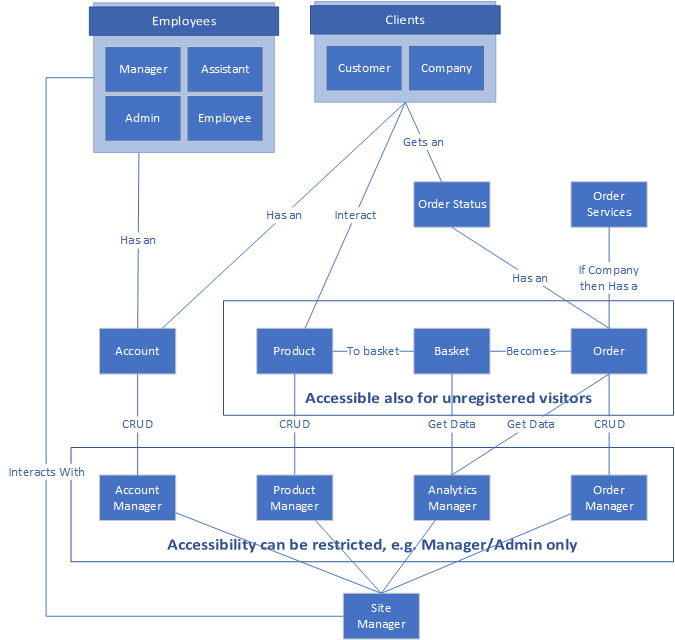
\includegraphics[width=1\textwidth]{figures/diagrams/dmd-start.png}
    \caption{Domain Model Diagram ved projektets start}
    \label{fig:appendix-domain-model-diagram}
\end{figure}

\section{Designklassediagrammer}
\label{appendix:class-diagrams}

\begin{figure}
    \centering
    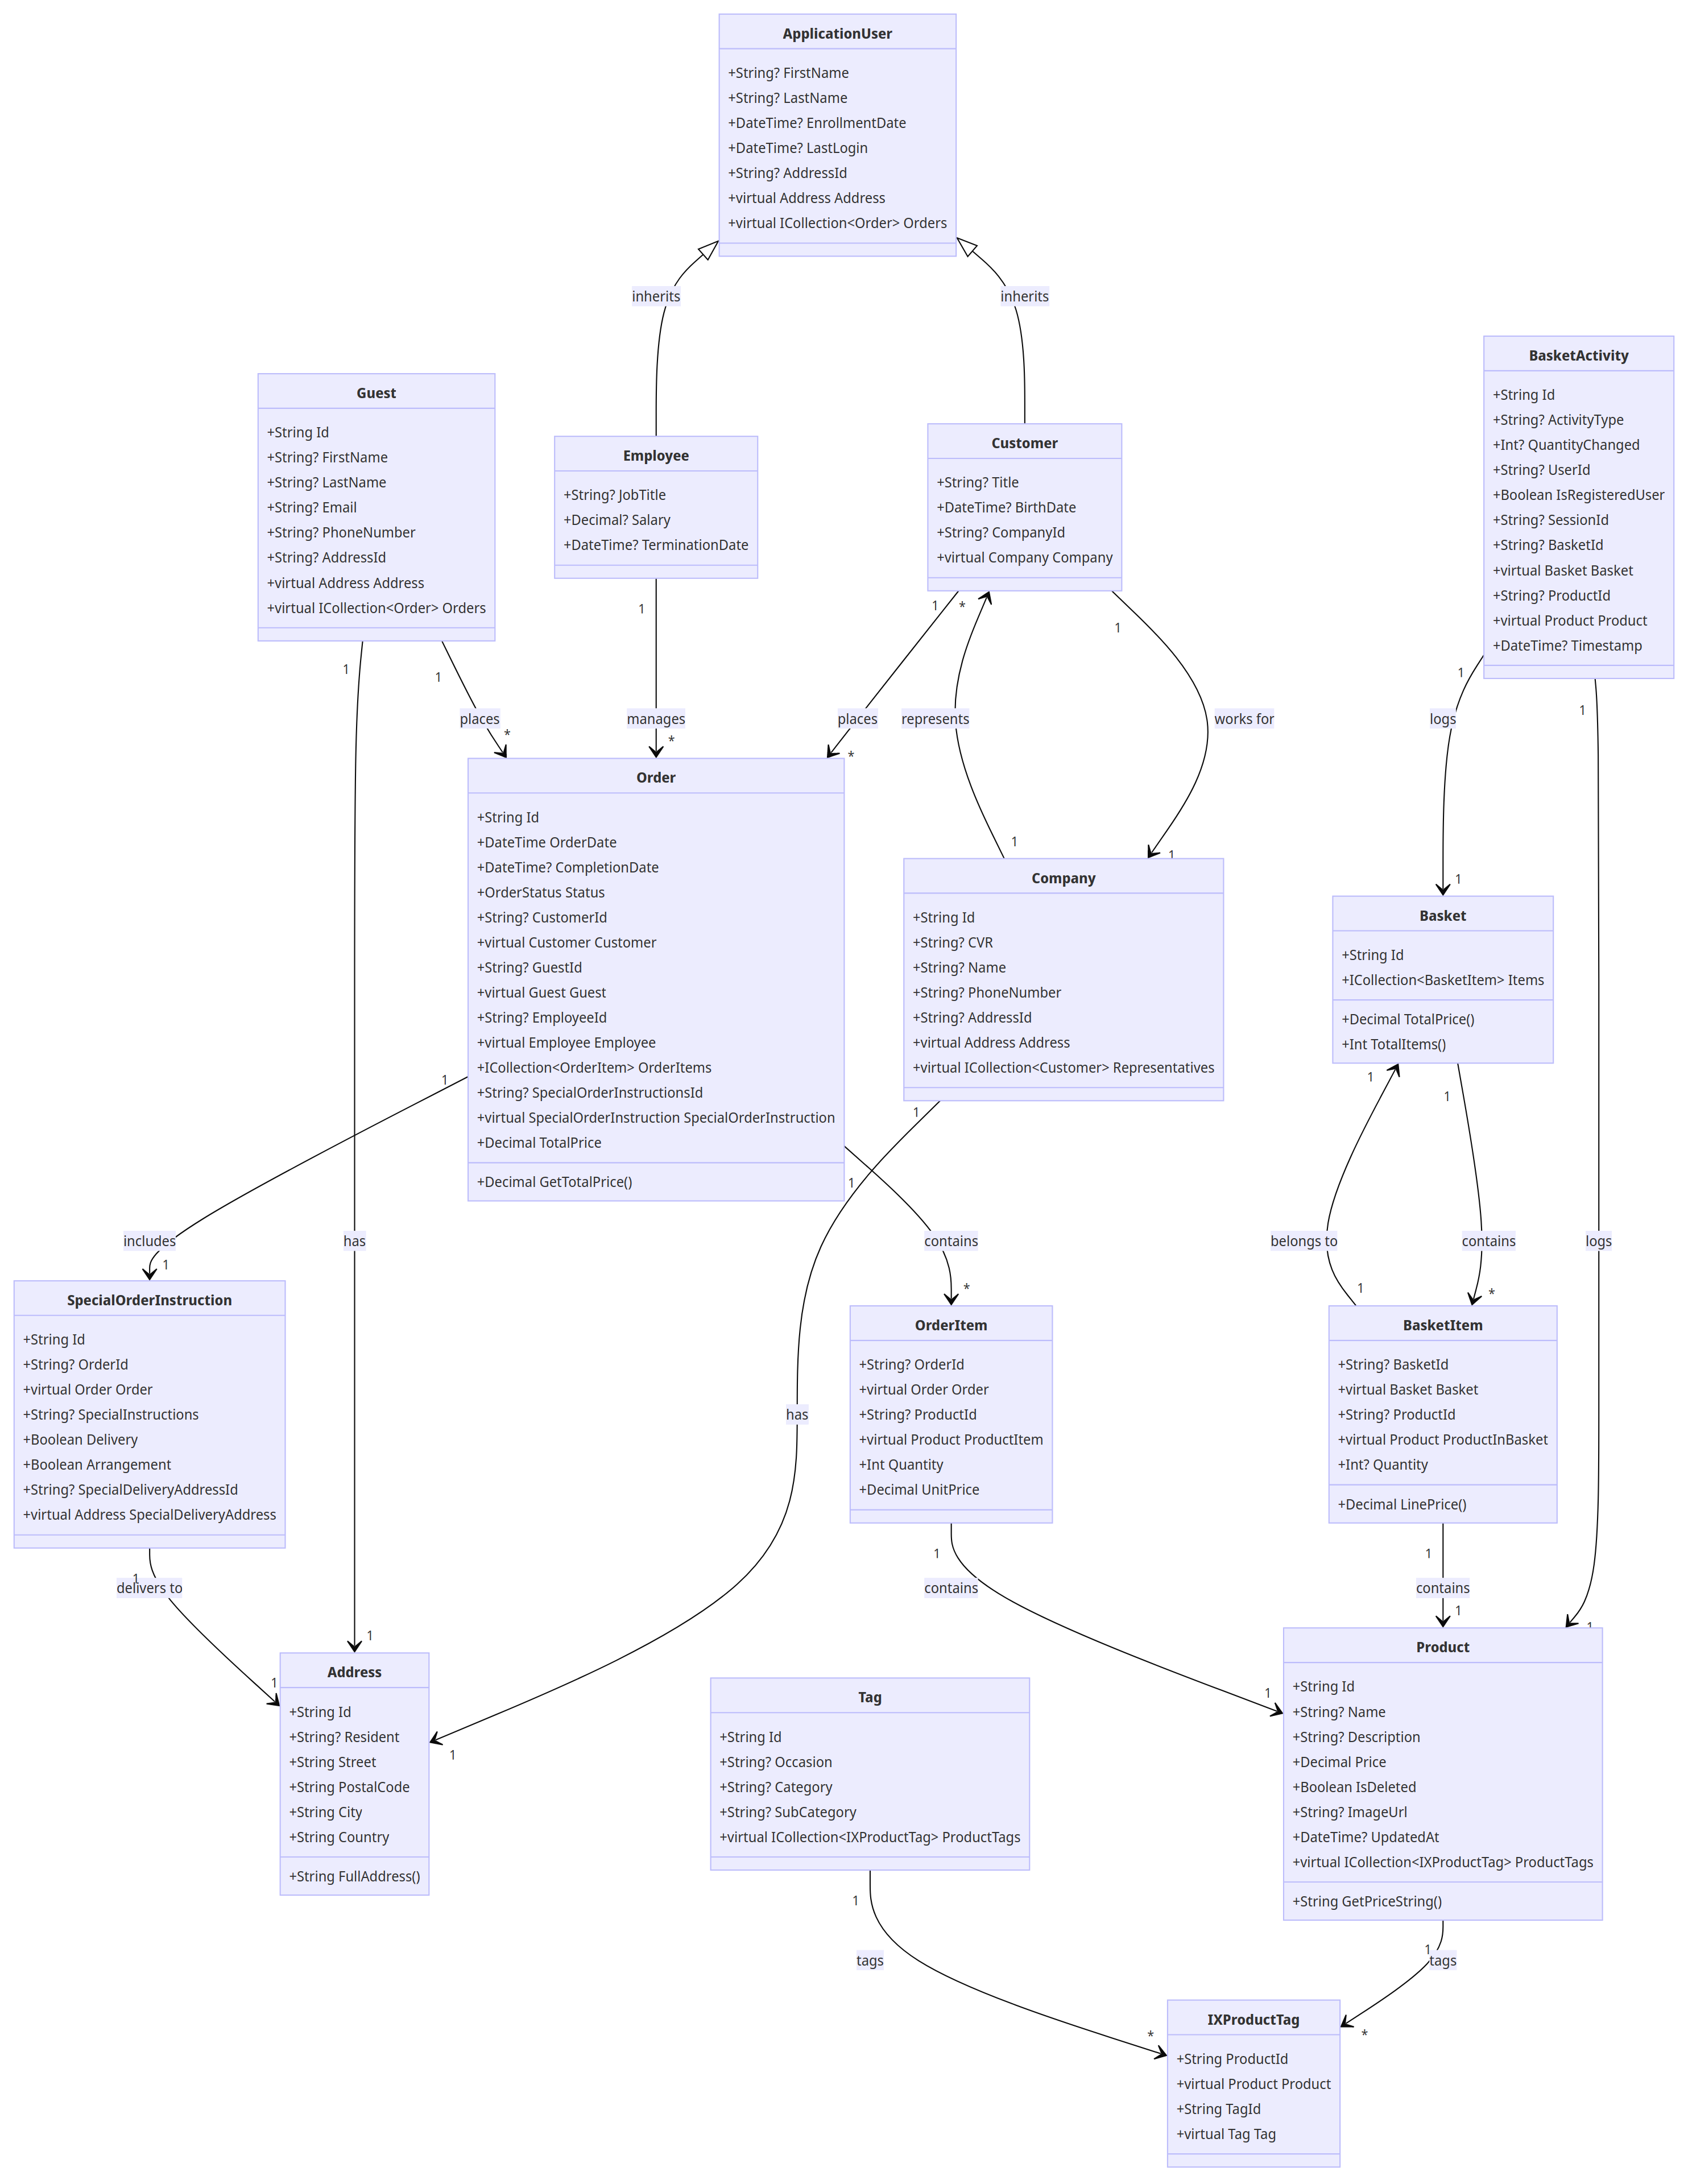
\includegraphics[width=1\textwidth]{figures/diagrams/dcd-modelclasses.png}
    \caption{Design Class Diagram - Model Classes}
    \label{fig:class-diagram-models}
\end{figure}

\begin{figure}
    \centering
    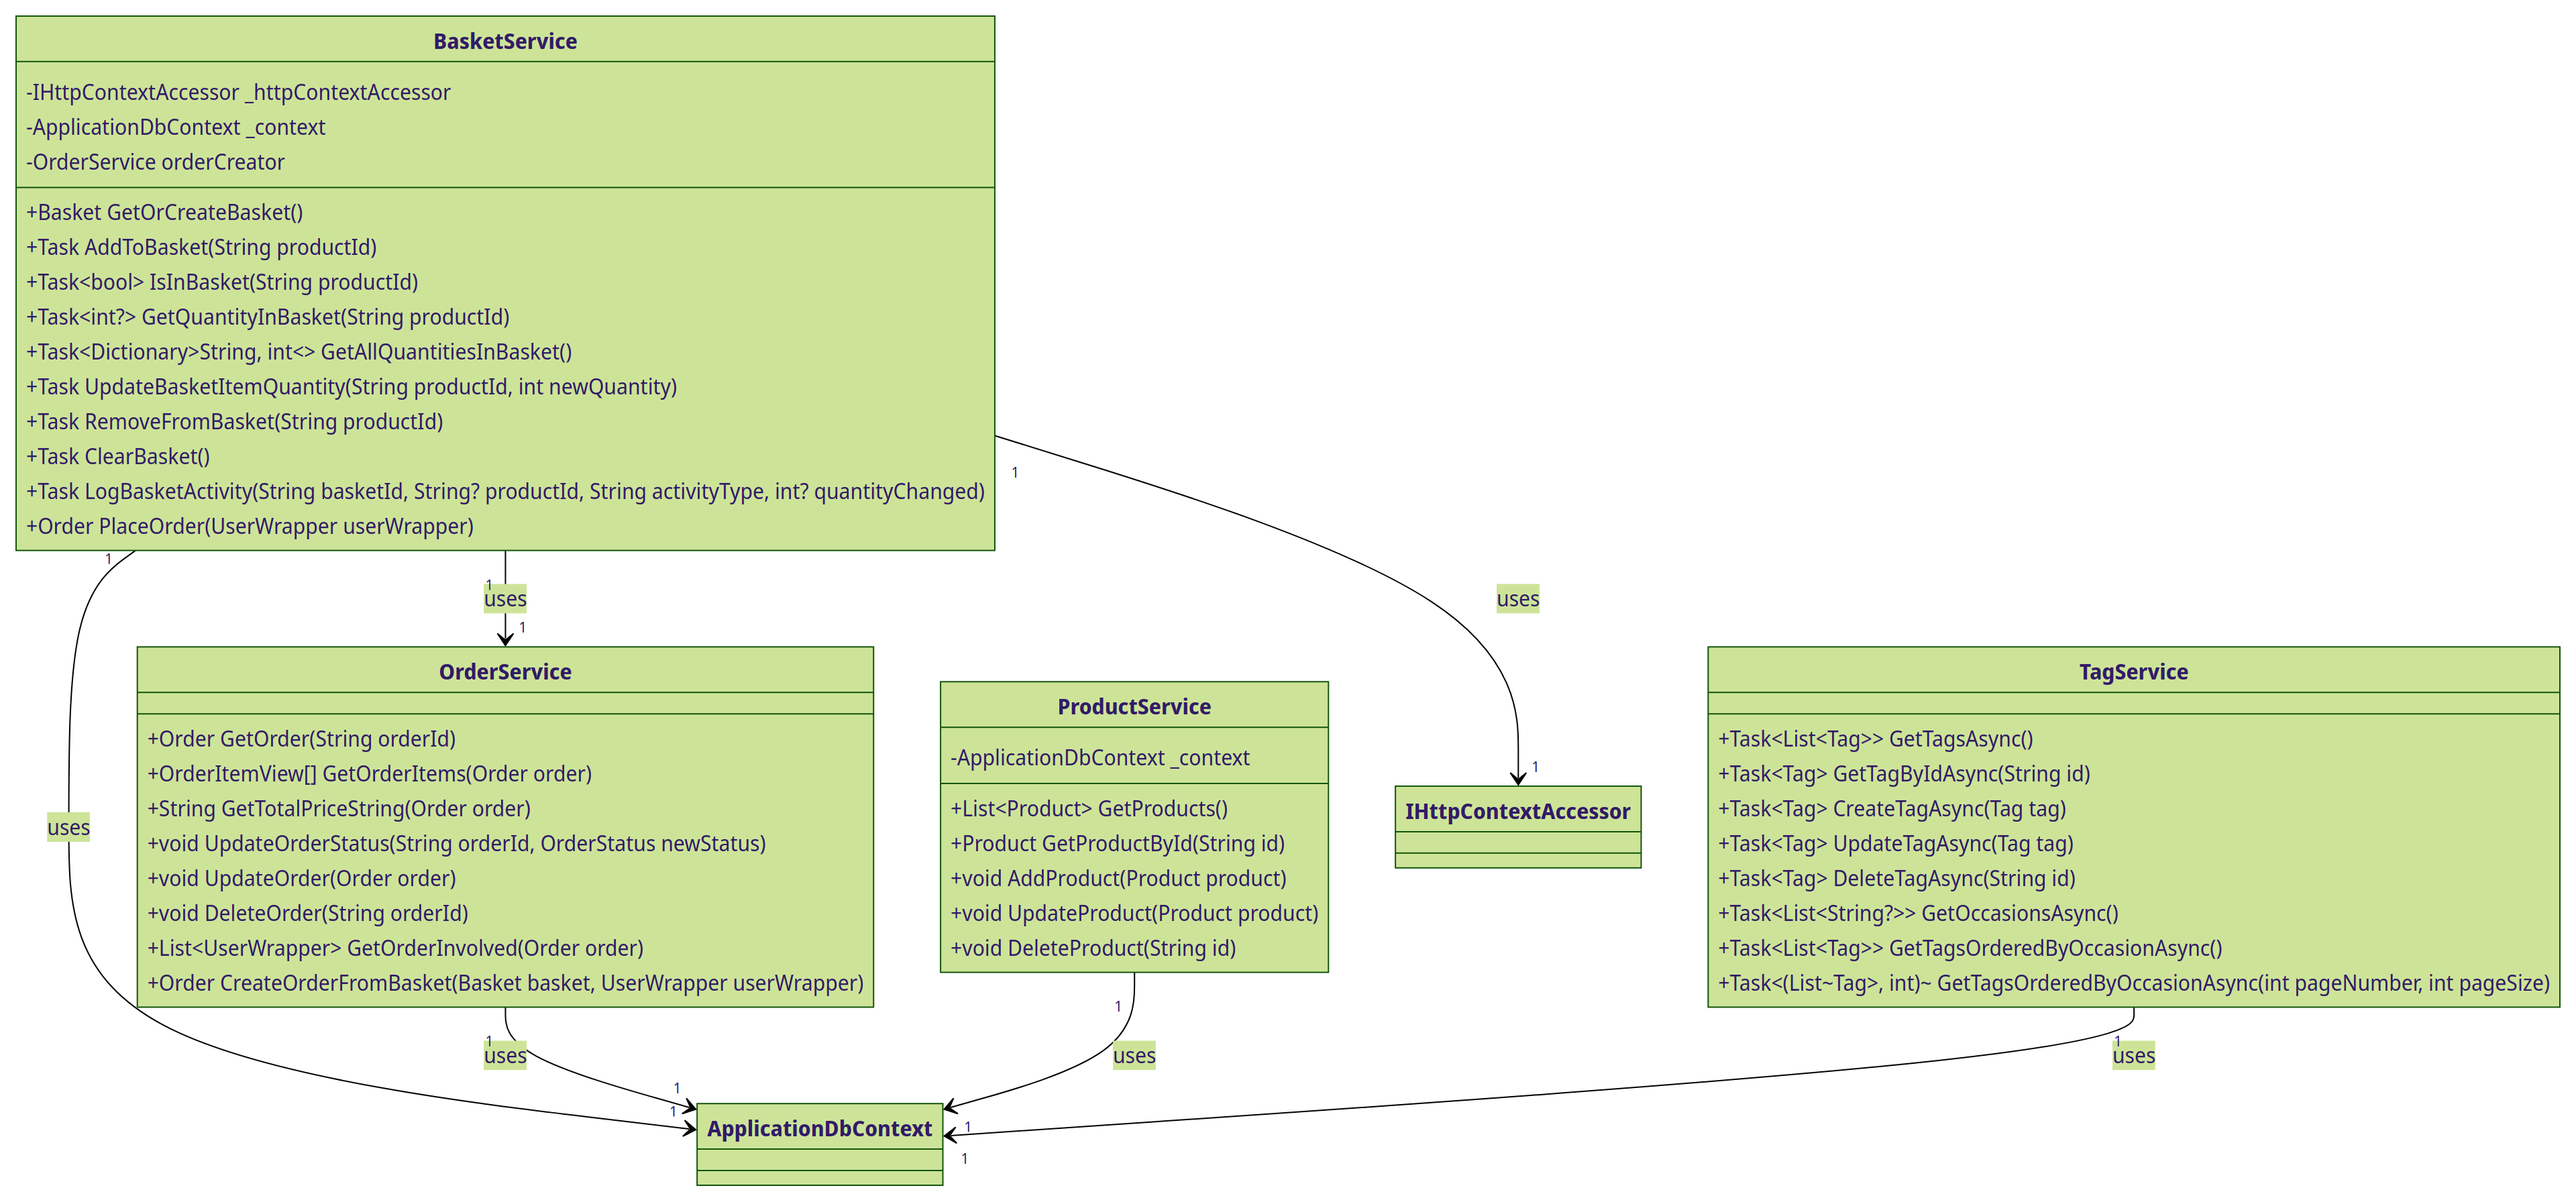
\includegraphics[width=1\textwidth]{figures/diagrams/dcd-main-services.png}
    \caption{Design Class Diagram - Main Services}
    \label{fig:class-diagram-main-services}
\end{figure}

\section{Database Diagrammer}

\subsection{Entity Relationship Diagrammer}
\label{appendix:entity-relationship-diagrams}
\begin{figure}
    \centering
    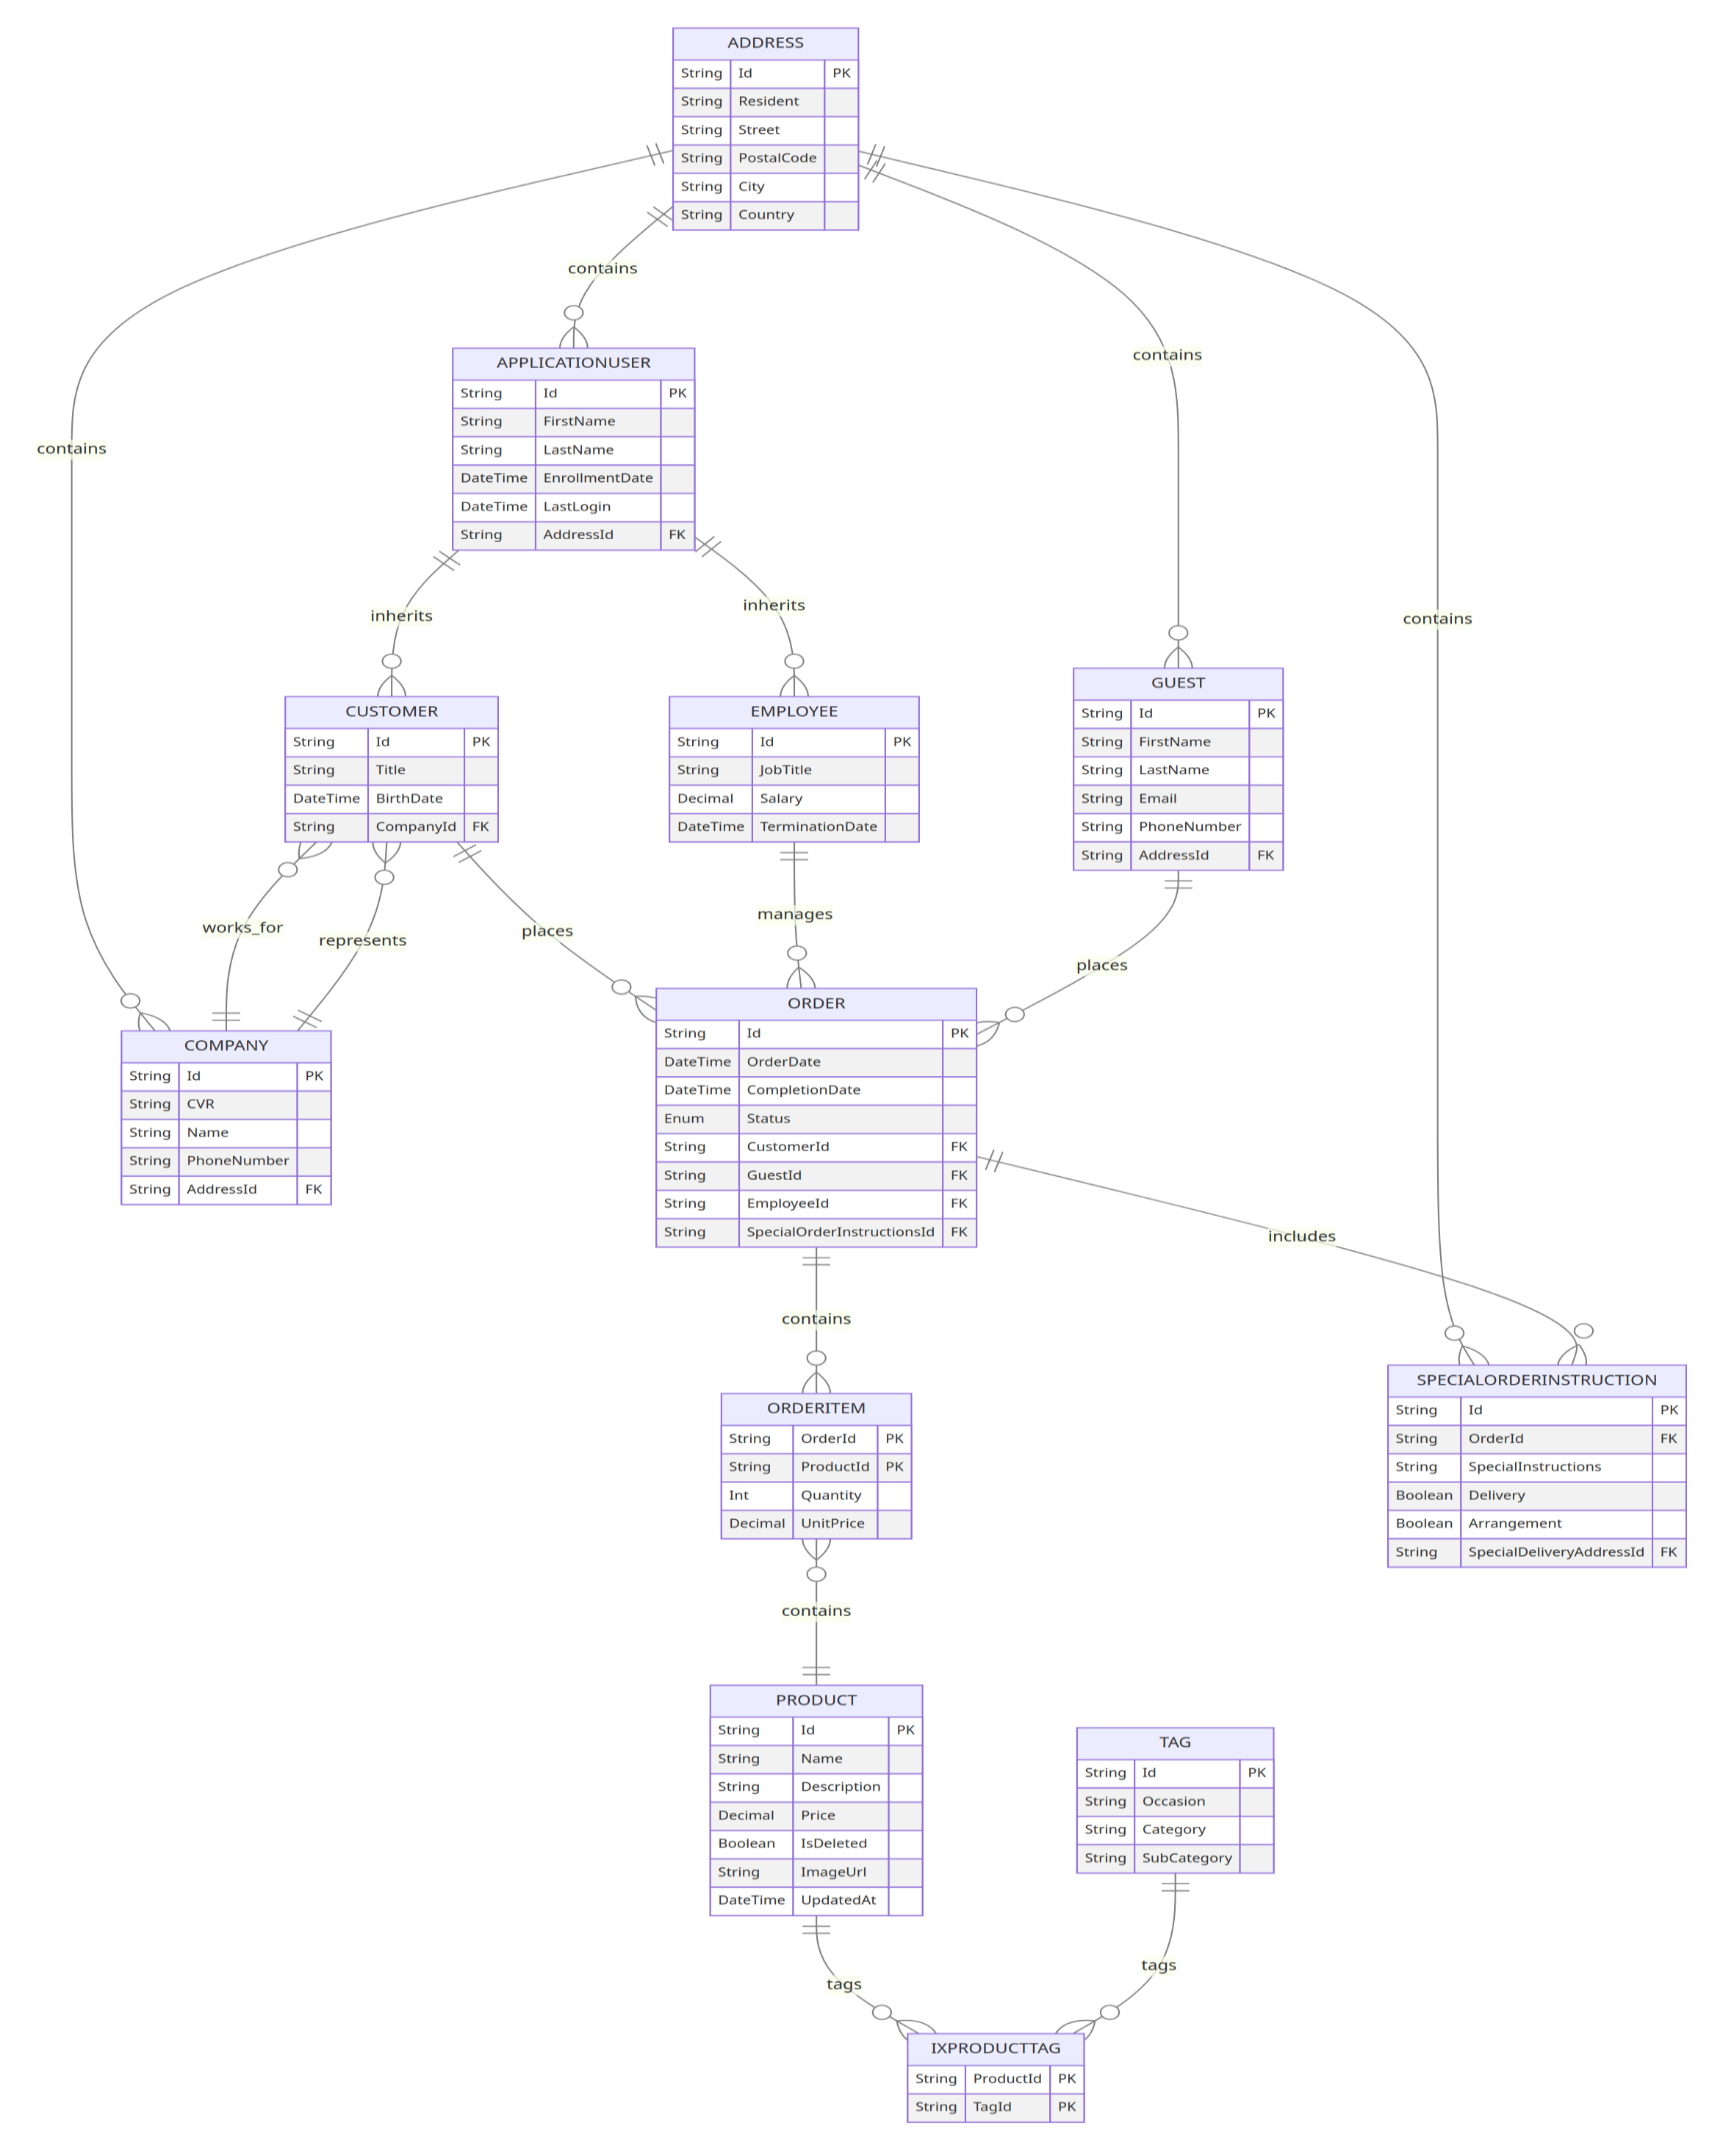
\includegraphics[width=1\textwidth]{figures/diagrams/erd-db-without-basket.png}
    \caption{Entity Relationship Diagram uden basket-relaterede entiteter}
    \label{fig:entity-relationship-diagram-nobasket}
\end{figure}

\section{Sekvensdiagrammer}
\label{appendix:sequence-diagrams}
\begin{figure}
    \centering
    \includegraphics[width=1\textwidth]{figures/diagrams/ssd-admin-updates-product-details.png}
    \caption{System Sequence Diagram - Admin Updates Product Details}
    \label{fig:ssd-admin-updates-product-details}
\end{figure}

\begin{figure}
    \centering
    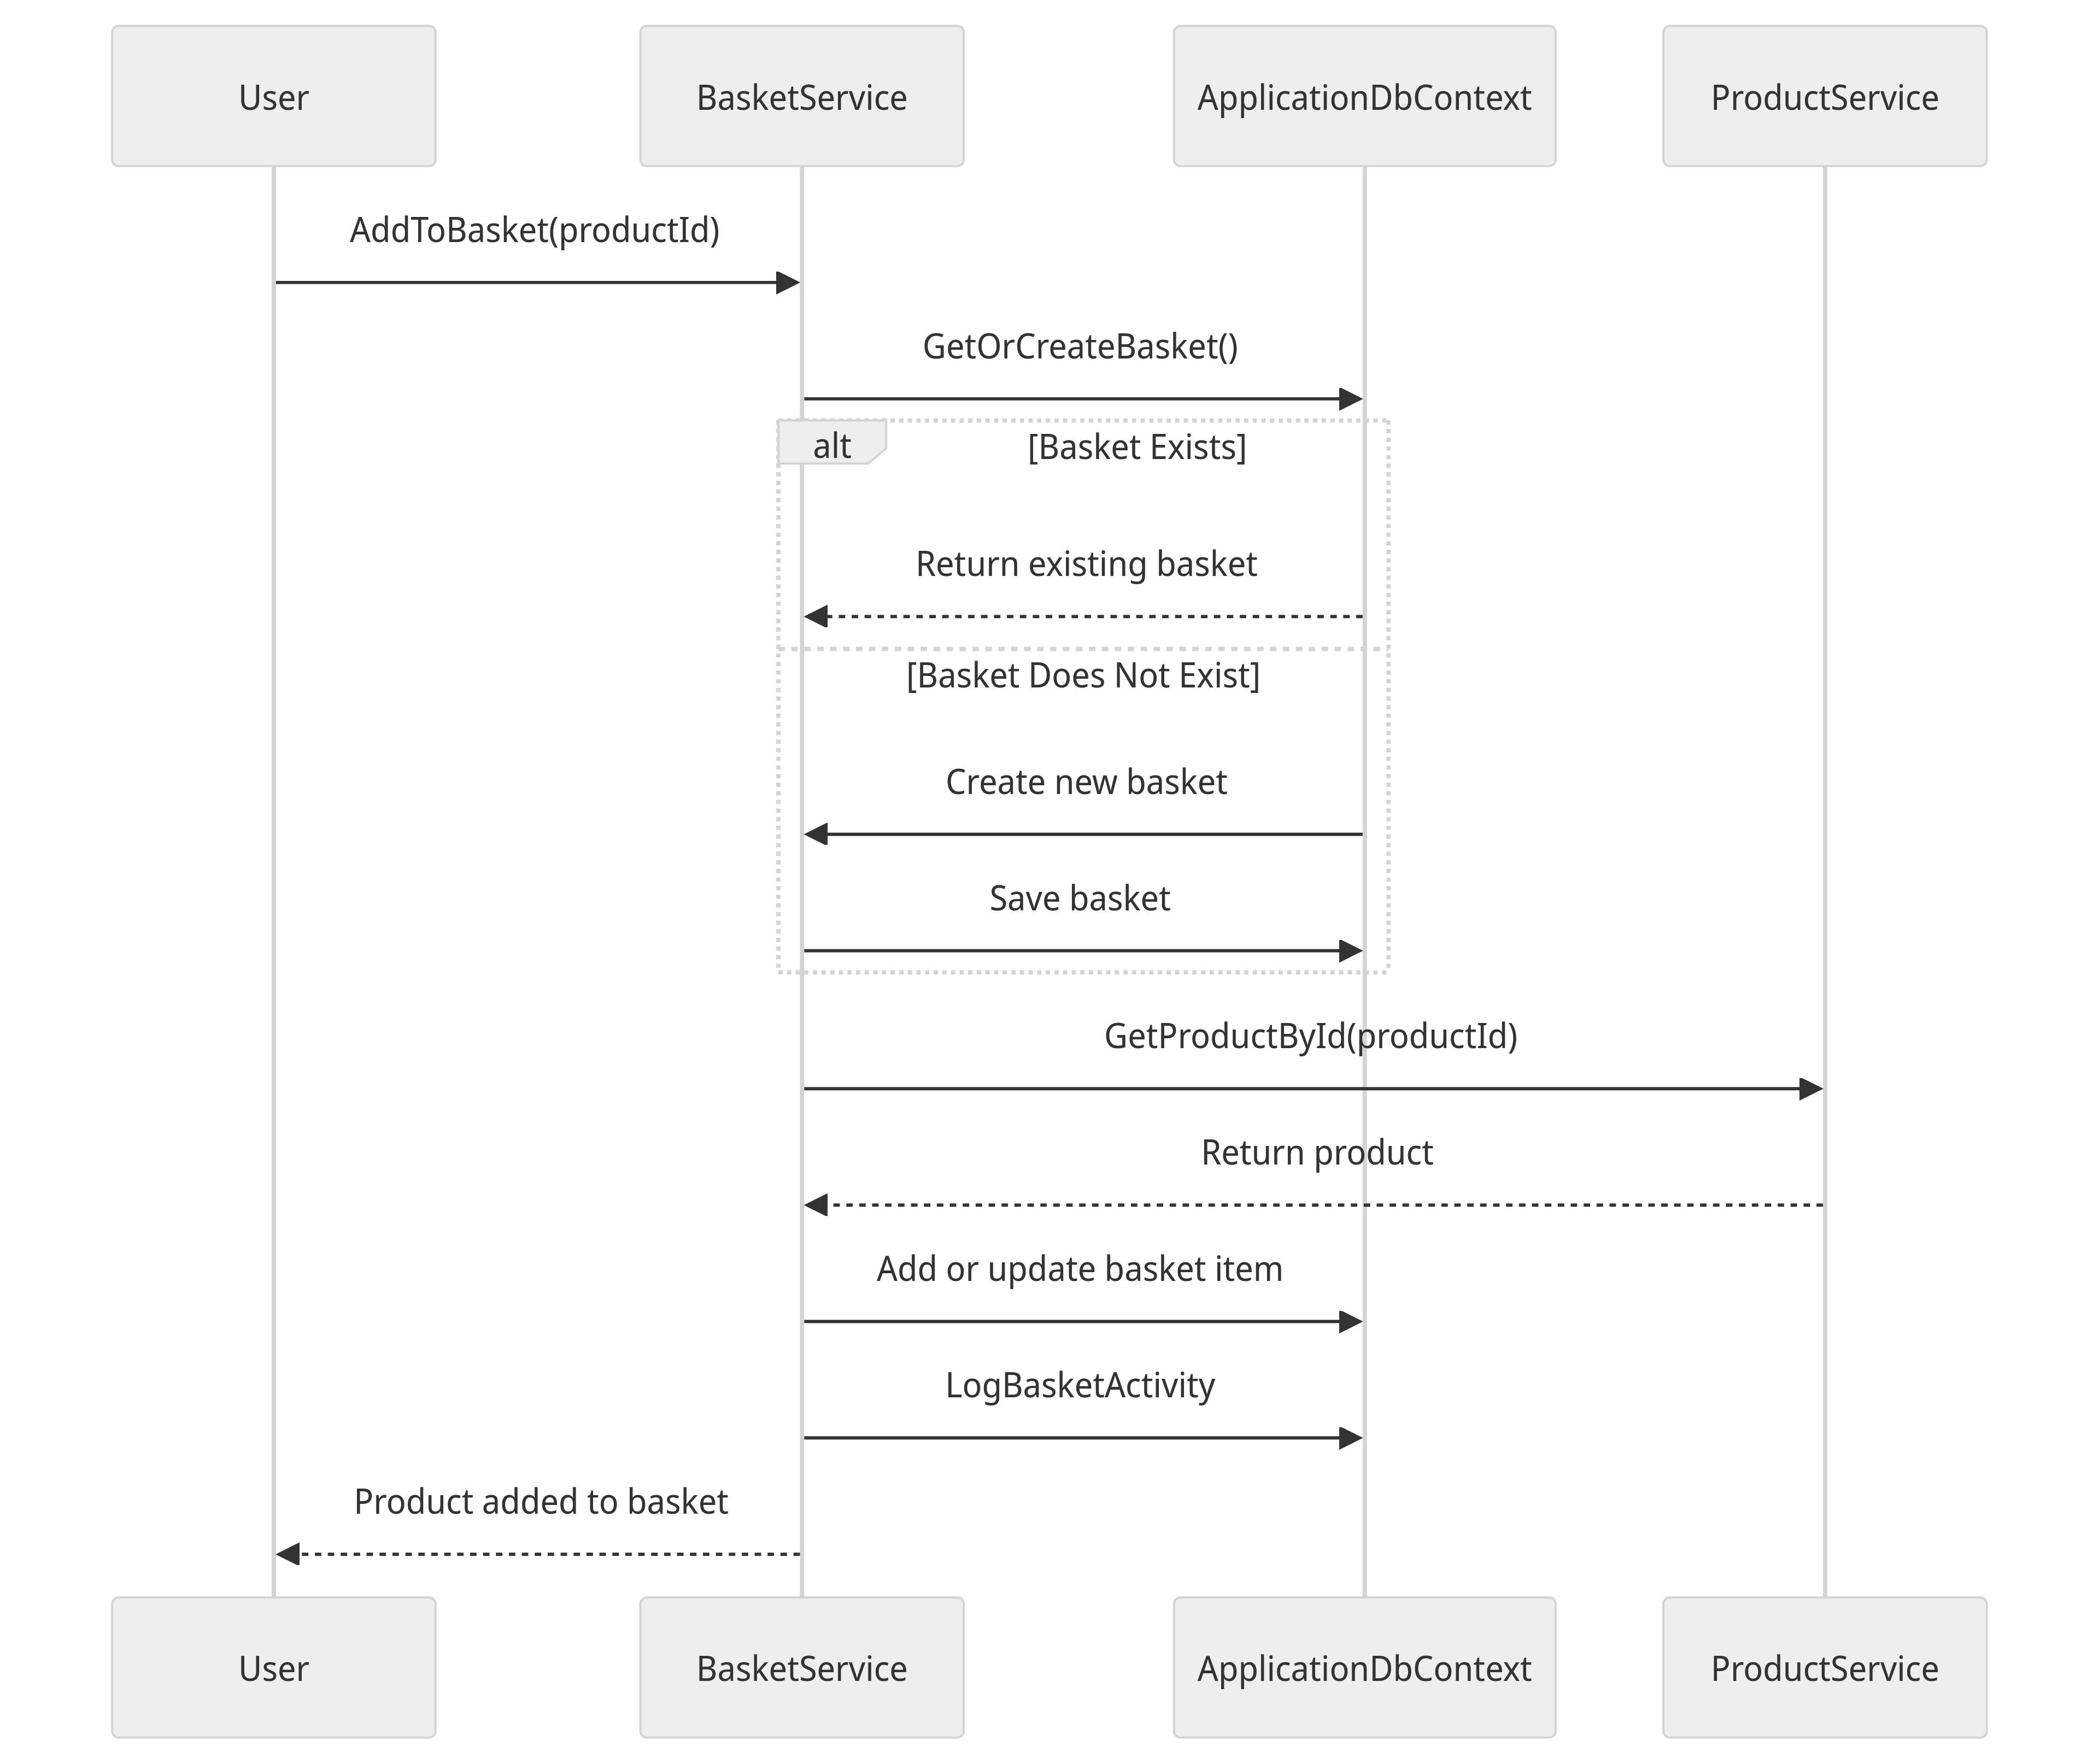
\includegraphics[width=1\textwidth]{figures/diagrams/ssd-user-adds-product-to-basket.png}
    \caption{System Sequence Diagram - User Adds Product to Basket}
    \label{fig:ssd-user-adds-product-to-basket}
\end{figure}
\chapter{Sourcecode}
\label{appendix:sourcecode}

\section{Modeller}

\subsection{Some models}
\label{subsection:user-model}

\inputminted{csharp}{codefiles/models/ApplicationUser.cs}
\label{minted:application-user}

\section{Scripts}

\subsection{GitHub scripts}
\label{appendix:github-scripts}
\begin{figure}
    \inputminted{yaml}{codefiles/build.yml}
    \caption{\emph{GitHub Workflows Build}}
    \label{minted:build-yml}
\end{figure}
\input{appendix/appendix-lib.tex}
\input{appendix/appendix-doxygen.tex}

\end{document}